\subsection{How Developers Develop Features\\ \textit{T. Girba, O. Greevy, S. Ducasse (CSMR'2007)}}

In 2007 the same team published this paper\cite{Girba2007}, on a similar subject as the previous. This time, they shifted their focus towards ownership of features as well as files. Indeed, the standard point of view, i.e ownership of packages, is how developers think about their code. However domain analysts and users are more likely to think in terms of features. Studying this metric could be useful to link the external and functionnal aspect of a project with its internal structure.
The visualisation displays the ownership of files within the project's features, which are also structurally linked. The following image is a representation of this visualisation on a program that is designed to manage a mobile phone:

\begin{figure}[H]
\centering
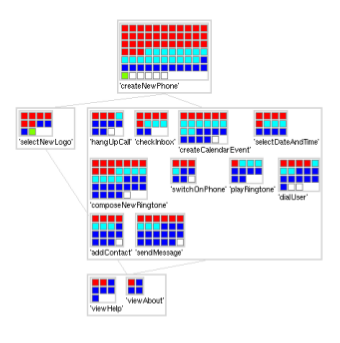
\includegraphics[width=0.4\textwidth]{./resources/girba2007.png}~
\caption{Ownership map By Feature}
\label{fig:ownership_map_by_feature}
\end{figure}

This visualisation makes it possible to determine whom one might ask in order to help resolve a bug in a feature, rather than having to identify which file belongs to which feature, as one would need to do with the previous paper's visualisation.
The goal was also to determine if developers tend to develop features or functionnal blocks. They determined that project contributions were mainly distributed on a package boundary.~\ref{fig:annex_ownership_outsight}.
